\section{Teil 2: Wellenlänge}
  In diesem Versuchsteil gilt es die geneue Wellenlänge der Cadmium-Linie zu bestimmen, Wir nutzen dazu zunächst das Spektrum einer Neon-Lampe als Referenz.
  Wir bestimmen wie zuvor mit \textbf{JImage} und \textbf{Python} die Position der Linien mit Hilfe eines Gauss-Fits.

  Das aufgenommene Spektrum von sowohl der Neon-Lampe, als auch das Cadmium Spektrum sind in \hyperref[plt::5]{Abb. \ref*{plt::5}} zu sehen. Aus welchem die folgenden Referenzwerte genutzt wurden:
  \begin{align}
    \lambda_{Ne,1} = \SI{633.443}{\nano\metre}\nonumber\\
    \lambda_{Ne,2} = \SI{638.299}{\nano\metre}\nonumber\\
    \lambda_{Ne,3} = \SI{640.225}{\nano\metre}\nonumber\\
    \lambda_{Ne,4} = \SI{650.623}{\nano\metre}\nonumber\\
    \lambda_{Ne,5} = \SI{653.288}{\nano\metre}\nonumber\\
    \lambda_{Ne,6} = \SI{659.895}{\nano\metre}
  \end{align}


  \begin{figure}[H]
    \centering
    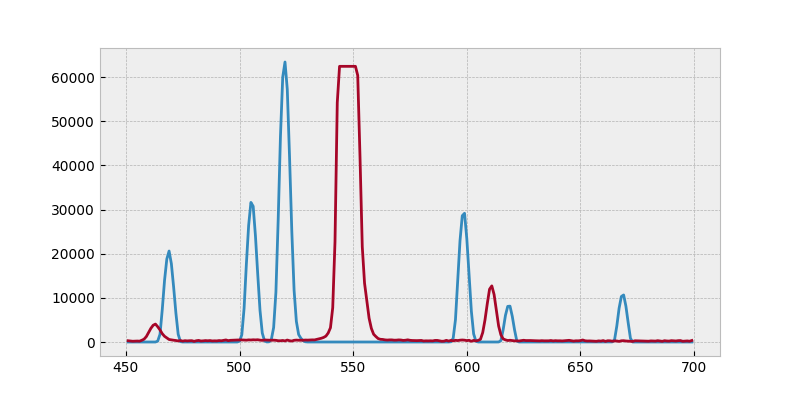
\includegraphics[width=\textwidth]{Auswertung/wavelength_analysis/wl}
    \caption{Cadmium- (Rot) und Neon- (Blau) Linien, y-Achse arbiträr}
    \label{plt::5}
  \end{figure}

  \subsection{Cadmium-Linie}
    Aus den so bestimmten Werten ergibt sich der folgende Zusammenhang (\hyperref[plt::6]{Abb. \ref*{plt::6}}), für Position und Wellenlänge, sowie die Wellenlänge der Cadmium-Linie.
    \begin{align}
      a_{Cd}       &= \SI{547.945+-4.310}{px}\\
      \lambda_{Cd} &= \SI{643.927+-0.571}{\nano\metre}
    \end{align}

    \subsection{unbekannte Linie}
      In unserem Spektrum sollte sich eine weitere Linie befinden, welche bei etwa $\SI{643}{\nano\metre}$ zu erkennen sei. Wir haben zwar eine weitere Linie rechts der Cd-Linie aufgenommen, diese befindet sich allerdings bei
      \begin{align}
        \lambda = \SI{652.253+-0.269}{nm}
      \end{align}
      und nicht bei \SI{646.494}{nm} oder \SI{672.578}{nm}
      %TODO: src https://physics.nist.gov/PhysRefData/Handbook/Tables/cadmiumtable2.htm



    \begin{landscape}
      \thispagestyle{empty}
      \begin{figure}
        \vspace*{-2cm}
        \caption{title}
        \hspace*{-6cm}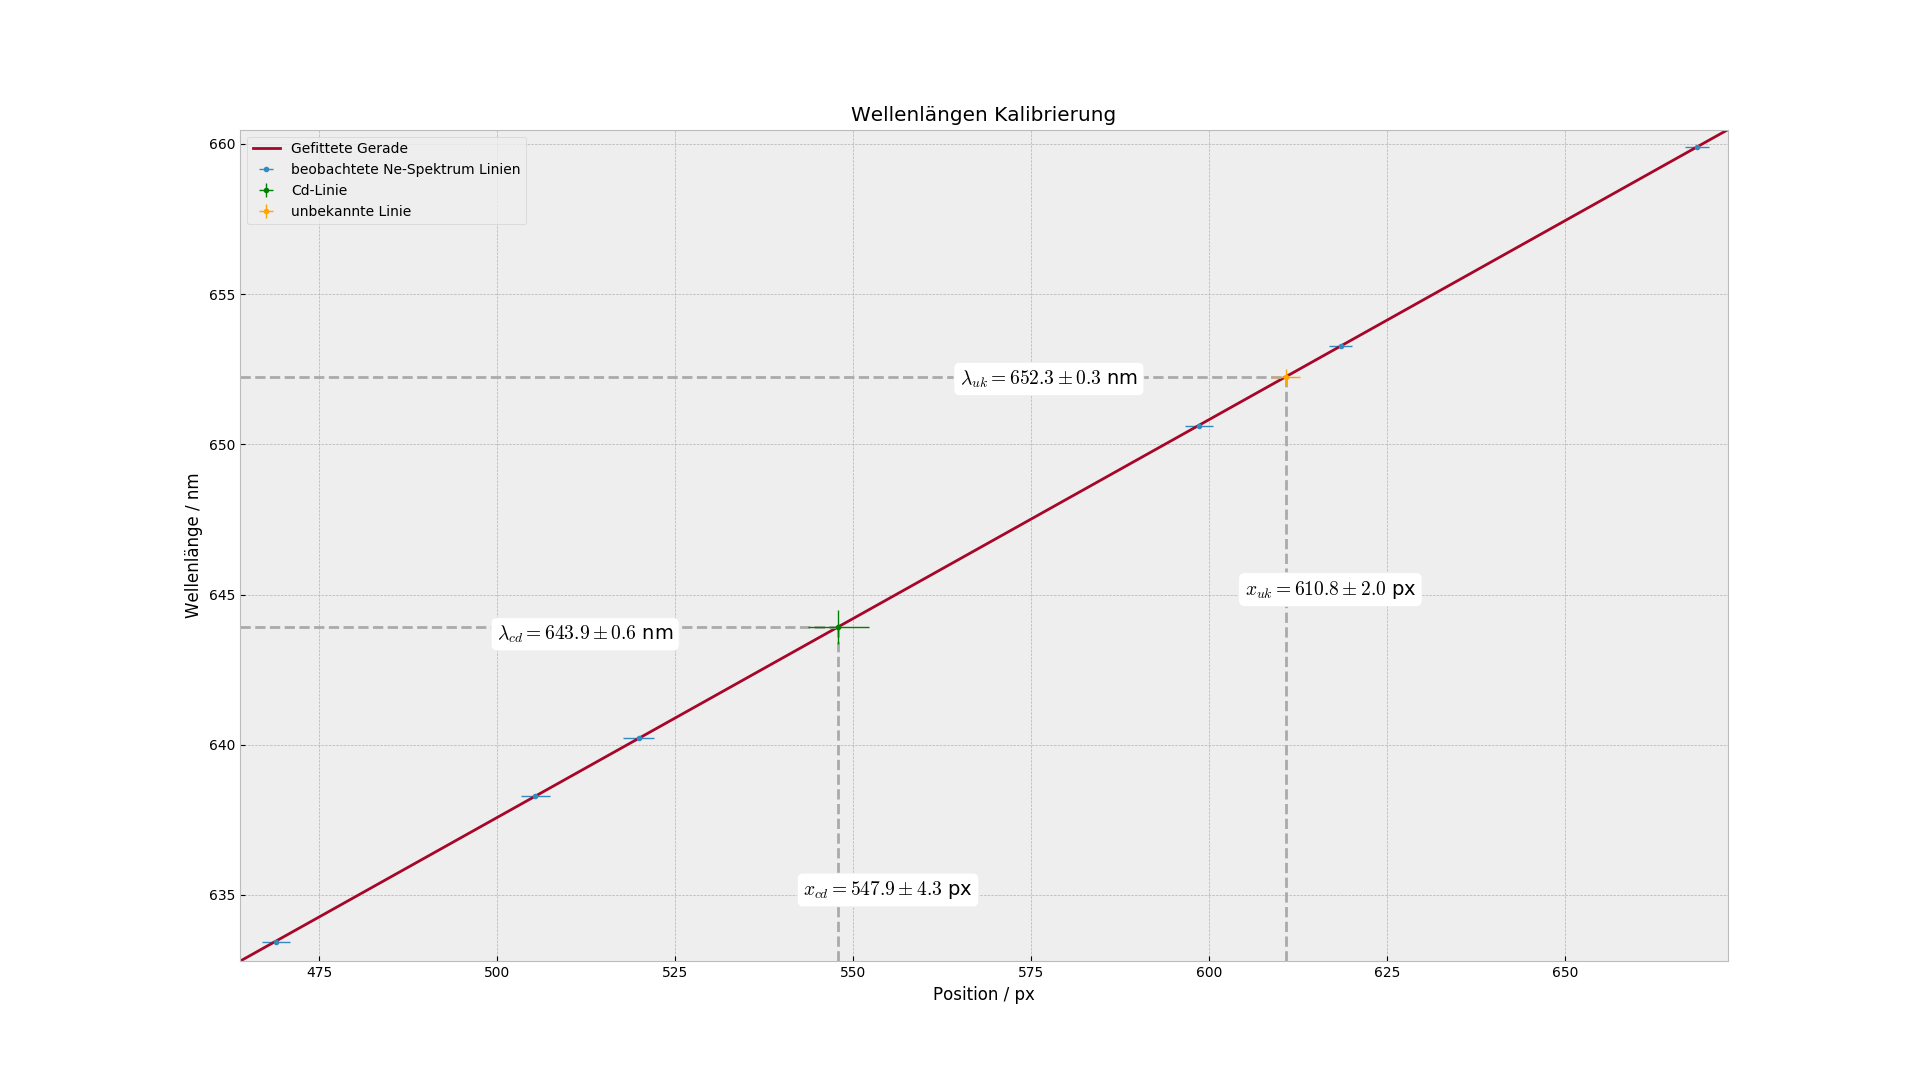
\includegraphics[width=1.5\paperwidth]{Auswertung/wavelength_analysis/wl_ne_cal}
        \label{plt::6}
      \end{figure}
    \end{landscape}
